\documentclass{beamer}

\usepackage[utf8]{inputenc}
\usepackage[square]{natbib}
\usepackage{ragged2e}

\renewcommand{\bibsection}{\subsubsection*{\bibname }}

\setbeamertemplate{caption}[numbered]
\renewcommand{\figurename}{Figura}
\renewcommand{\tablename}{Tabela}

\usetheme{Madrid}
\usecolortheme{default}
\useoutertheme{miniframes}

%------------------------------------------------------------
%This block of code defines the information to appear in the
%Title page
\title[] % (optional)
{Predição da geração de energia utilizando dados climáticos}

\author[Vitor~Oliveira~Ropke] % (optional)
{
    Vitor~Oliveira~Ropke
}

\institute[] % (optional)
{
    
\includegraphics[height=1.5cm]{brasao-uern.png}
    \hspace{3cm}
    
\includegraphics[height=1.5cm]{logo-ppgcc.png}
    \hspace{3cm}
    
\includegraphics[height=1.5cm]{brasao-ufersa.eps}
}

\date[Dezembro de 2024] % (optional)
{Dezembro de 2024}

%End of title page configuration block
%------------------------------------------------------------


\begin{document}

%Hide the navigation buttons
\beamertemplatenavigationsymbolsempty

%The next statement creates the title page
\frame{\titlepage}

%---------------------------------------------------------


\section{Introdução}


%---------------------------------------------------------
\begin{frame}
\frametitle{Mudanças climáticas}
\begin{itemize}
    \item Baseado no modelo aditivo
    \item Funciona melhor com dados sazonais
    \item Trata dados faltantes, mudanças de padrões e outliers
\end{itemize}
\end{frame}
%---------------------------------------------------------


%---------------------------------------------------------
\begin{frame}
\frametitle{Sistema Interligado Nacional (SIN)}
\begin{equation}
    y(t) = g(t) + s(t) + h(t) + \epsilon_t
\end{equation}
\begin{itemize}
    \item $y(t)$: Função resultante.
    \item $g(t)$: Função de tendência.
    \item $s(t)$: Função de sazonalidade.
    \item $h(t)$: Função de feriados.
    \item $\epsilon_t$: Mudanças idiossincráticas.
\end{itemize}
\end{frame}
%---------------------------------------------------------


%---------------------------------------------------------
\begin{frame}
\frametitle{Componentes}
\begin{figure}
    \centering
    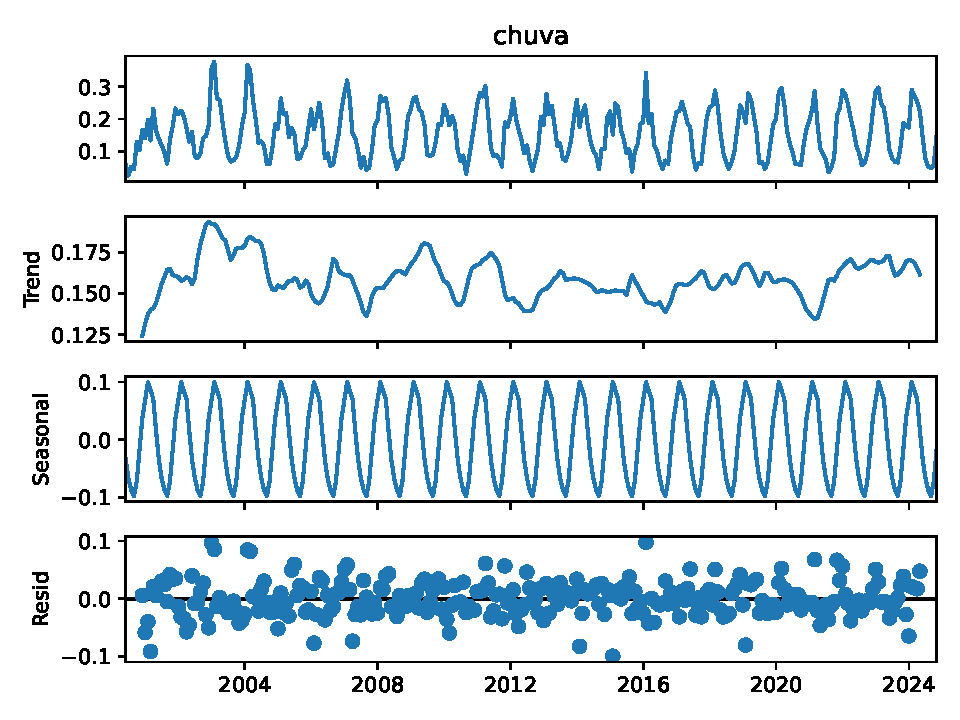
\includegraphics[width=0.6\linewidth]{componentes-modelo-aditivo.pdf}
    \caption{Componentes de um Modelo Aditivo}
\end{figure}
\end{frame}
%---------------------------------------------------------


%---------------------------------------------------------
\begin{frame}
\frametitle{Tendência}
A incerteza da previsão é definida através da seguinte equação:

\begin{equation}
    \lambda = \frac{1}{S} \sum_{j=1}^S |\delta_j|
\end{equation}

\begin{itemize}
    \item $\lambda$: Incerteza da previsão.
    \item $S$: Número de mudanças na tendência.
    \item $|\delta_j|$: Valor da mudança na tendência.
\end{itemize}
\end{frame}
%---------------------------------------------------------


%---------------------------------------------------------
\begin{frame}
\frametitle{Tendência}

\begin{figure}
    \centering
    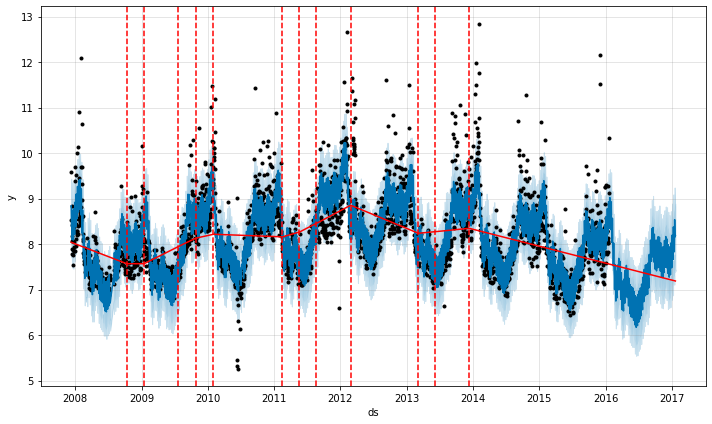
\includegraphics[width=0.8\linewidth]{tendencia.png}
    \caption{Tendência em uma Série Temporal}
\end{figure}
\end{frame}
%---------------------------------------------------------


%---------------------------------------------------------
\begin{frame}
\frametitle{Sazonalidade}
A sazonalidade é feita a partir da série de Fourier, dada na seguinte equação:

\begin{equation}
    s(t) = \sum_{n=1}^N \left( a_n cos \left( \frac{2 \pi nt}{P} \right) + b_n sin \left( \frac{2 \pi nt}{P} \right) \right)
\end{equation}

\begin{itemize}
    \item $N$: Número de termos de Fourier (filtro passa-baixa).
    \item $P$: Regularidade do período em número de dias.
\end{itemize}
\end{frame}
%---------------------------------------------------------


%---------------------------------------------------------
\begin{frame}
\frametitle{Sazonalidade}
\begin{figure}
    \centering
    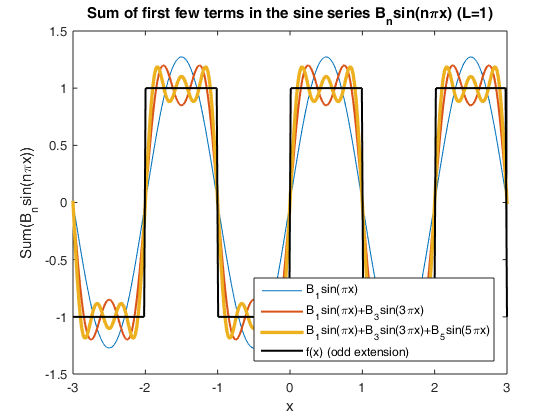
\includegraphics[width=0.6\linewidth]{fourier.png}
    \caption{Séries de Fourier}
\end{figure}
\end{frame}
%---------------------------------------------------------


%---------------------------------------------------------
\begin{frame}
\frametitle{Sazonalidade}

\begin{figure}
    \centering
    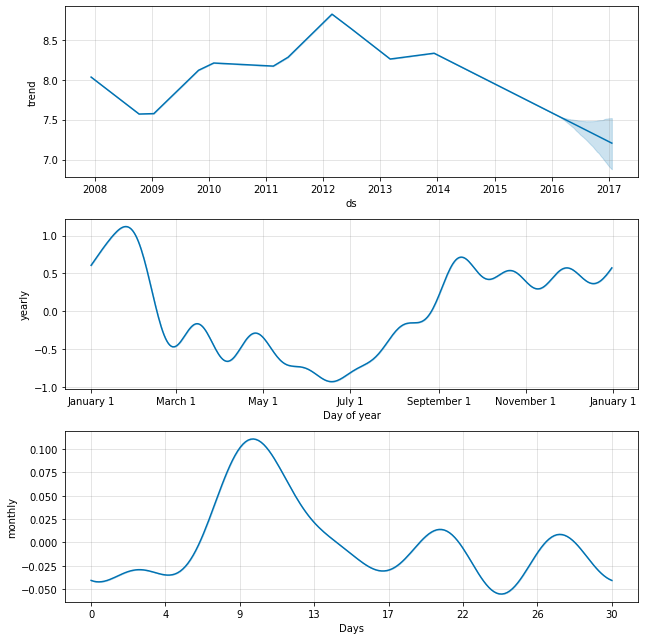
\includegraphics[width=0.4\linewidth]{sazonalidade.png}
    \caption{Sazonalidade de uma Série Temporal}
\end{figure}
\end{frame}
%---------------------------------------------------------


\section{Modelo Híbrido}


%---------------------------------------------------------
\begin{frame}
\frametitle{NeuralProphet}
\begin{itemize}
    \item Além de redes neurais, utiliza outros modelos de \textit{deep learning}
    \item É uma extensão do Prophet
\end{itemize}
\end{frame}
%---------------------------------------------------------


%---------------------------------------------------------
\begin{frame}
\frametitle{Componentes}
\begin{equation}
    \hat{y}(t) = T(t) + S(t) + E(t) + F(t) + A(t) + L(t)
\end{equation}
\begin{itemize}
    \item $\hat{y}(t)$: Valores preditos.
    \item $T(t)$: Função de tendência.
    \item $S(t)$: Função de sazonalidade.
    \item $E(t)$: Função de eventos e feriados.
    \item $F(t)$: Efeitos de regressão para variáveis externas com futuro conhecido.
    \item $A(t)$: Efeitos de auto-regressão baseados nas observações passadas.
    \item $L(t)$: Efeitos de regressão para as últimas observações de variáveis exógenas.
\end{itemize}
\end{frame}
%---------------------------------------------------------


%---------------------------------------------------------
\begin{frame}
\frametitle{Auto-regressão}
O cálculo de valores futuros é feito usando a seguinte equação:

\begin{equation}
    y_t = c + \sum_{i=1}^{i=p} \theta_i \cdot y_{t-i} + \epsilon_t
\end{equation}
\begin{itemize}
    \item $y_t$: Valor predito.
    \item $p$: Número de valores passados.
    \item $\theta_i$: Coeficiente a direção e magnitude do valor passado $i$.
    \item $c$: Interceptor.
    \item $\epsilon_t$: Ruído branco.
\end{itemize}
\end{frame}
%---------------------------------------------------------


%---------------------------------------------------------
\begin{frame}
\frametitle{Auto-regressão}

\begin{figure}
    \centering
    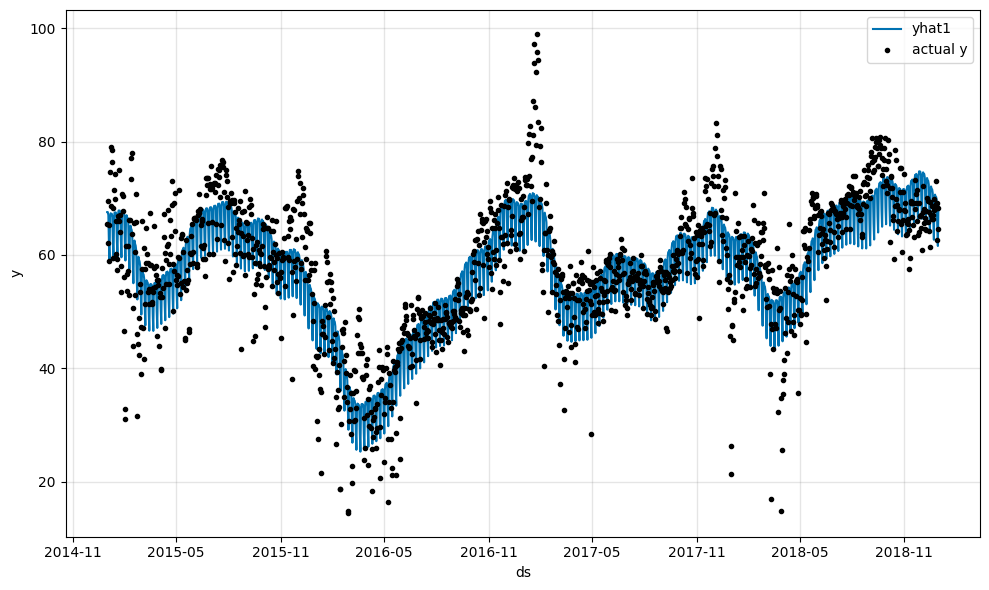
\includegraphics[width=0.8\linewidth]{auto-regressao.png}
    \caption{Auto-regressão comparado com valores reais}
\end{figure}
\end{frame}
%---------------------------------------------------------


%---------------------------------------------------------
\begin{frame}
\frametitle{Regressores defasados (\textit{Lagged Regressors})}
Usado para correlacionar outras variáveis (covariáveis) com o target, seguindo a equação:

\begin{equation}
    L(t) = \sum_{x \in \mathbb{X}} L_x (x_{t-1}, x_{t-2}, \cdots, x_{t-p})
\end{equation}
\begin{itemize}
    \item $L(t)$: Valor defasado.
    \item $\mathbb{X}$: Conjunto das covariáveis.
    \item $x$: Valor da covariável.
\end{itemize}
\end{frame}
%---------------------------------------------------------


%---------------------------------------------------------
\begin{frame}
\frametitle{Regressores defasados (\textit{Lagged Regressors})}
\begin{figure}
    \centering
    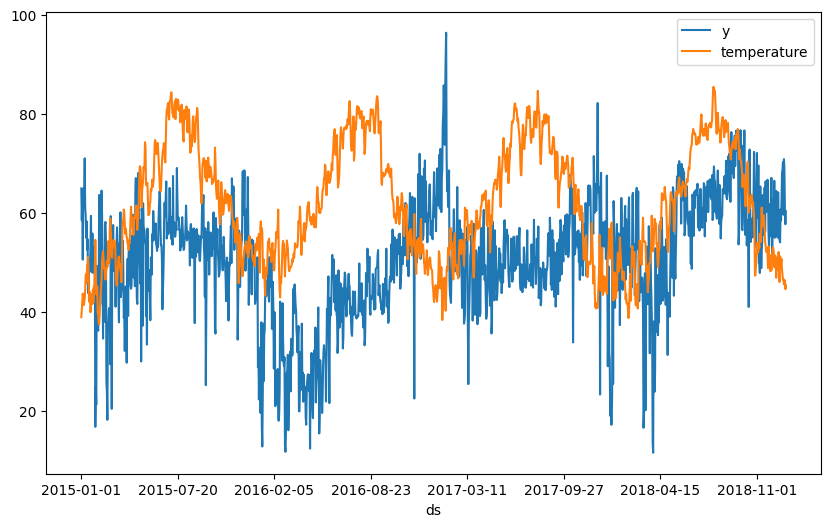
\includegraphics[width=0.7\linewidth]{regressores-defasados.png}
    \caption{Covariável e target}
\end{figure}
\end{frame}
%---------------------------------------------------------


%---------------------------------------------------------
\begin{frame}
\frametitle{Regressores do futuro}
Covariáveis com futuro conhecido, seguindo a equação:

\begin{equation}
    F(t) = \sum_{f \in \mathbb{F}} F_f^\star(t)
\end{equation}
\begin{itemize}
    \item $F(t)$: Efeito de todos os regressores.
    \item $\mathbb{F}$: Conjunto das covariáveis com futuro conhecido.
    \item $f$: Regressor.
\end{itemize}
\end{frame}
%---------------------------------------------------------


%---------------------------------------------------------
\begin{frame}
\frametitle{Regressores do futuro}
\begin{figure}
    \centering
    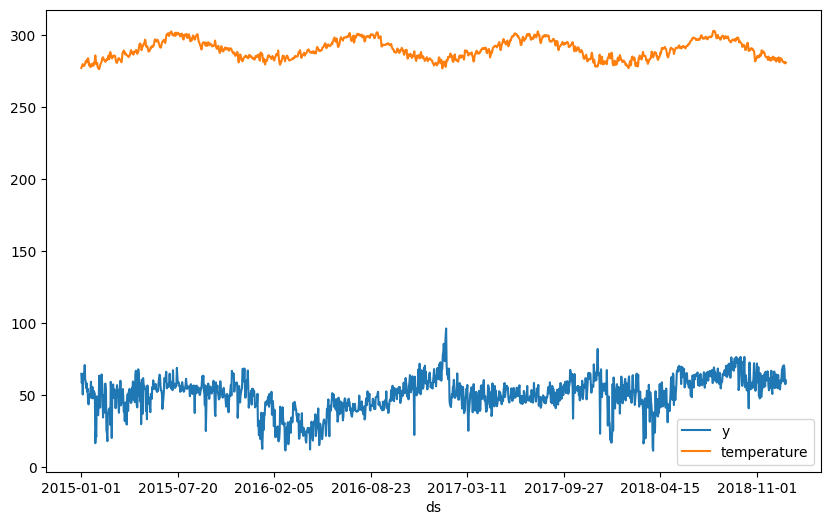
\includegraphics[width=0.7\linewidth]{regressores-futuro.png}
    \caption{Covariável e target}
\end{figure}
\end{frame}
%---------------------------------------------------------


\section*{}
\setcounter{section}{0}


%---------------------------------------------------------
\begin{frame}
\begin{center}
    \Huge ACABOU-SE!!!
\end{center}
\begin{figure}
    \centering
    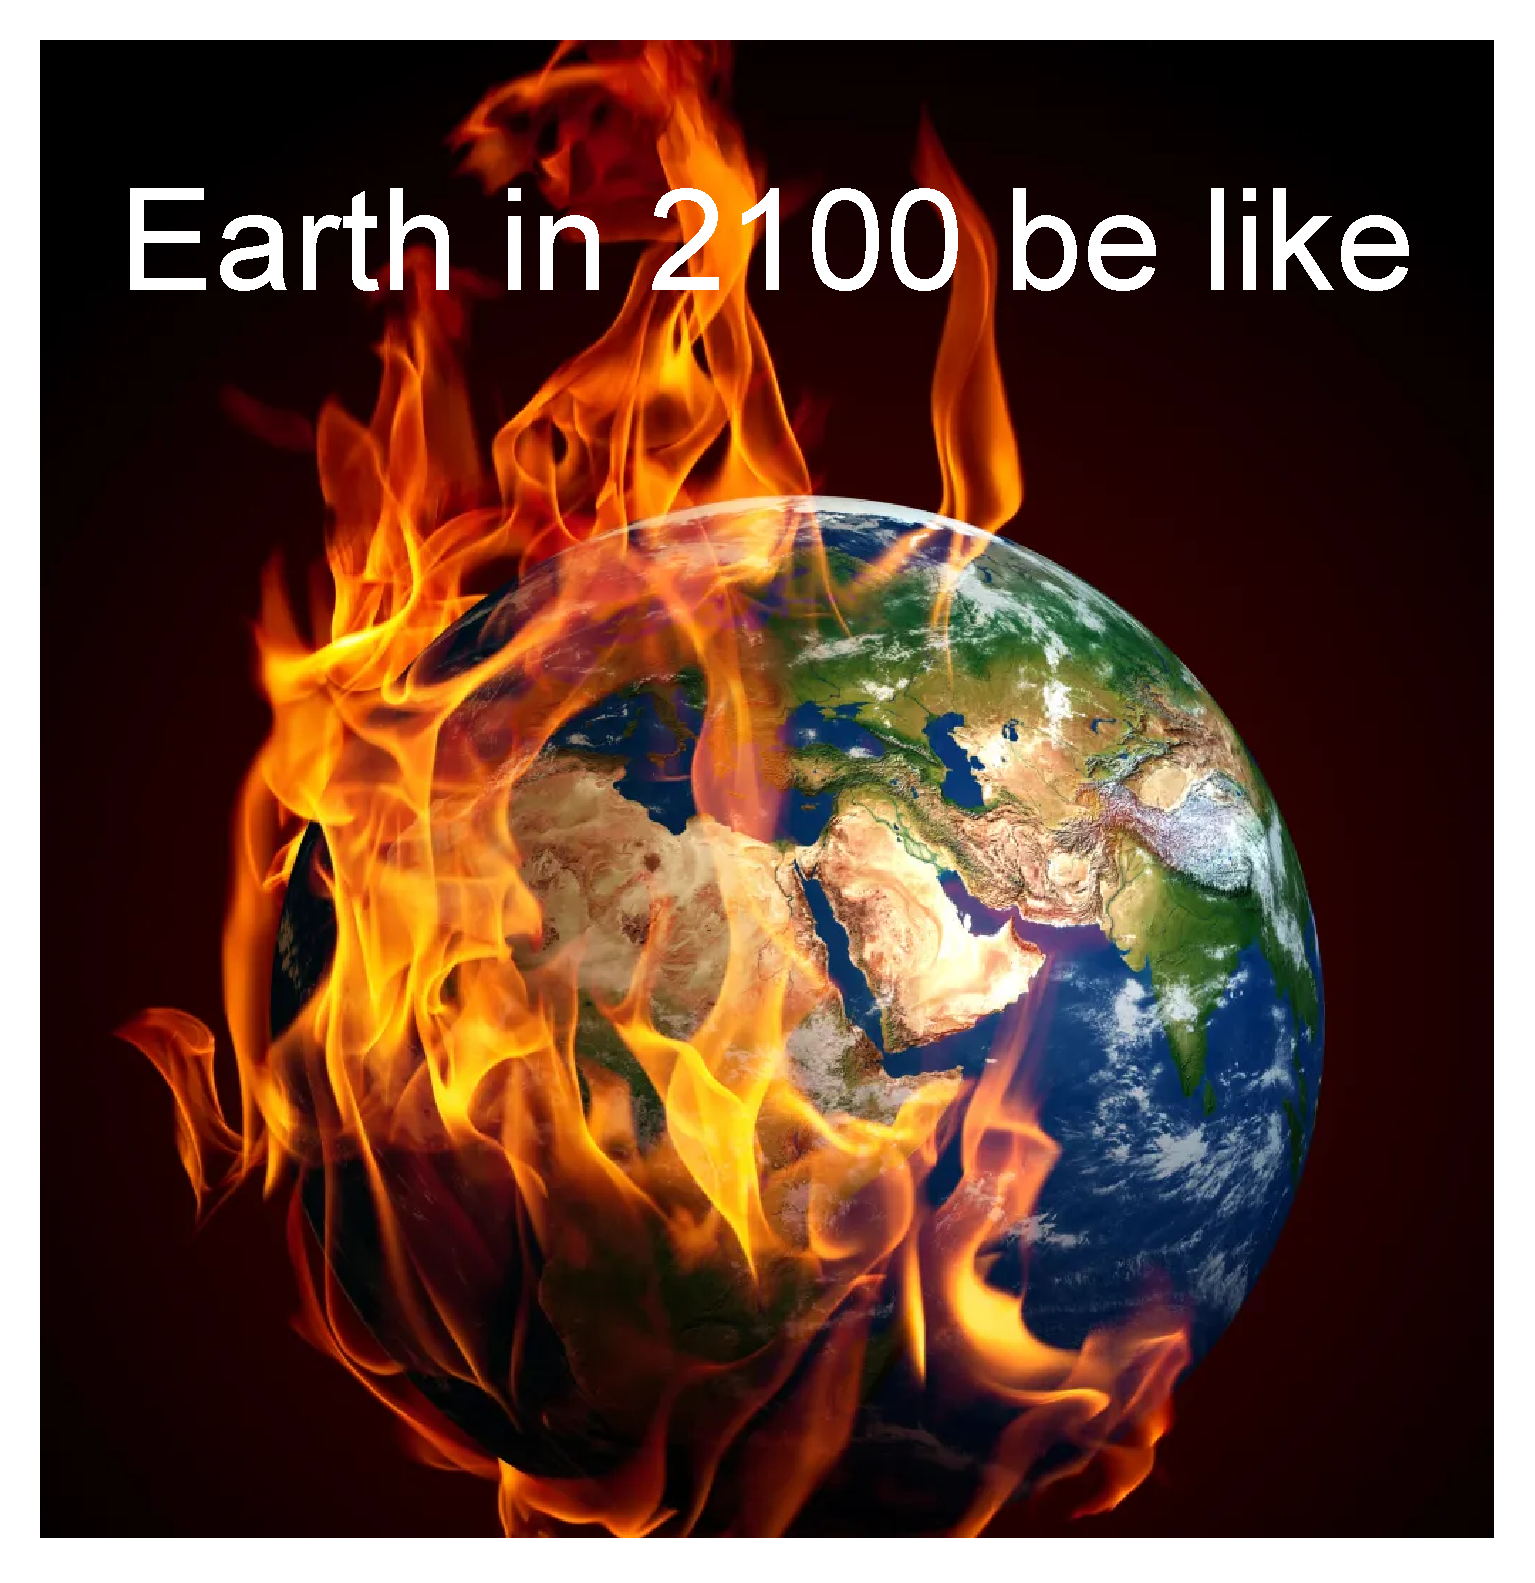
\includegraphics[width=0.5\linewidth]{earth-2100-be-like.pdf}
\end{figure}
\end{frame}
%---------------------------------------------------------


\end{document}
